\subsection{Equazioni differenziali lineari del I ordine}

\subsubsection{Definizione Integrale Generale}

Prendiamo una EDO lineare di I ordine in forma implicita:
\[
    F(x, y, y') = 0
\]

Consideriamo ora l'EDO in forma normale (1) e la sua omogenea associata (2):
\begin{align*}
    y'(x)+a(x)y(x) & = f(x) & \qquad \circled{1} \\
    y'(x)+a(x)y(x) & = 0    & \qquad \circled{2}
\end{align*}

dove \(x \in [a,b]\) e \(a(x), f(x)\) sono funzioni continue in \([a,b]\).

Attenzione, con il termine omogenea associata si intende un equazione separata che ha \(0\) come \(f(x)\); è sbagliato dire che \(f(x) = 0\).

Infatti, data una equazione in forma normale insieme alla sua omogenea associata, vogliamo studiare com'è possibile relazionarle per trovare l'insieme di tutte le soluzioni di (1).

\teorema{}{
L'integrale generale di (1) in \([a,b]\) è dato dalla somma dell'integrale generale dell'omogenea associata (2) con un integrale particolare di (1)
\[
    \underbrace{\int gen\,(1)}_{y(x)} = \underbrace{\int gen\,(2)}_{z(x)} + \underbrace{\int particolare\,(1)}_{\bar{y}(x)}
\]
}

Questo teorema vale per tutte le EDO lineari di ordine \(n\).

\begin{proof}
    Sia \(y(x)\) una soluzione qualsiasi di (1) (\(y(x)\) appartiene all'integrale generale di (1))
    e sia \(\bar y(x)\) una soluzione particolare (nota) di (1). Voglio far vedere è che la loro differenza è una soluzione qualsiasi di (2) \(= z(x)\).

    Dunque per ipotesi si ha che:
    \begin{align*}
         & y'(x)+a(x)y(x) = f(x)\ \ \ \forall x \in [a,b]              \\
         & \bar y'(x) + a(x) \bar y(x) = f(x)\ \ \ \forall x \in [a,b]
    \end{align*}

    Entrambe soddisfano la (1). Le sottraggo membro a membro:

    \begin{align*}
        y'(x)-\bar y'(x) + a(x)y(x) - a(x) \bar y(x)         & = f(x) - f(x) \\
        y'(x)-\bar y'(x) + a(x)\left[y(x) - \bar y(x)\right] & = 0
    \end{align*}

    e raccogliendo le derivate:
    \[
        [y(x)-\bar y(x)]' + a(x)[y(x) - \bar y(x)] = 0
    \]

    Dunque, la funzione \(y(x) - \bar y(x) = z(x)\) è soluzione di (2)
    Quindi:
    \[
        y(x) = \bar y(x) + z(x)
    \]

    Viceversa, se \(z(x)\) è una qualsiasi soluzione di (2) e \(\bar y(x)\) è una soluzione particolare di (1)
    voglio mostrare che la loro somma è soluzione di (1).

    Quindi, abbiamo:
    \begin{align*}
        z'(x) + a(x)z(x)            & = 0    \\
        \bar y'(x) + a(x) \bar y(x) & = f(x)
    \end{align*}

    e ponendo
    \[
        y(x) = z(x) + \bar y(x)
    \]
    bisogna dimostrare che \(y(x)\) verifica (1).

    Derivando ambo i membri e sviluppando:
    \begin{align*}
        (y(x))'                                                                  & = \left( z(x) + \bar{y}(x) \right)'                               \\
                                                                                 & = [z'(x)] + [\bar{y}'(x)]                                         \\
                                                                                 & = \left[ -a(x)z(x) \right] + \left[ -a(x)\bar y(x) + f(x) \right] \\
                                                                                 & = -a(x) \left[ z(x) + \bar y(x) \right] +f(x)                     \\
        \intertext{da cui:}
        \left( z(x) + \bar{y}(x) \right)'                                        & = -a(x) \left[ z(x) + \bar y(x) \right] +f(x)                     \\
        \left( z(x) + \bar{y}(x) \right)' + a(x) \left[ z(x) + \bar y(x) \right] & = f(x)                                                            \\
    \end{align*}
    dunque:
    \begin{align*}
         & \implies \bigl\lparen z(x) + \bar{y}(x) \bigr\rparen \ \text{è soluzione generale di (1)} \\
         & \implies y(x) \ \text{è soluzione generale di (1)}
    \end{align*}

\end{proof}

\subsubsection*{Validità del teorema per \texorpdfstring{\(n>1\)}{n>1}}

Supponiamo che \(u\) e \(v\) siamo due soluzioni di (1), cioè che:

\(Lu=f\) e \(Lv=f\) su \(I\)

La differenza di queste diventano soluzione su \(I=[a,b]\) dell'omogenea associata

Usando la proprietà della linearità:
\[
    L(\lambda u+\mu v) = \lambda L u + \mu L v
\]
possiamo dire che:
\[
    L(u-v) = Lu-Lv = f- f=0
\]

Se indichiamo con \(V_0\) l'insieme di tutte le soluzioni dell'equazione omogenea associata (\(Lw=0\) su \(I=[a,b]\) e \(V_0\) è l'insieme delle \(w \in C^n(I)\)) e con \(\bar u(t)\) una soluzione nota di (1)

\[
    u(x) = \bar u(x) +w(x)
\]

L'uguaglianza sopra, al variare di \(w(x)\) in \(V_0\) ci dà tutte le soluzioni del problema di partenza.

(Il problema quindi, diventa solo di studiare il problema omogeneo)

\subsubsection{Integrale generale dell'omogenea associata = z(x)}

Vediamo come si determina l'insieme di tutte le soluzioni di (2), ovvero l'integrale generale di:
\[
    y'(x)+a(x)y(x) = 0\ \ \ x \in [a,b] \qquad \circled{2}
\]

Sia \(A(x)\) una \textbf{primitiva} di \(a(x)\) su \(I = [a,b]\).

Sappiamo che (2) è continua su I, quindi è anche derivabile su I

\begin{align*}
    A'(x) & = a(x)              & \forall x \in [a,b] \\
    A(x)  & = \int a(x) \diff x & \forall x \in [a,b]
\end{align*}

Moltiplichiamo i due membri della (2) per la quantità sempre positiva \(e^{A(x)}\):

\begin{align*}
    e^{A(x)} y'(x) + e ^{A(x)}a(x) y(x) & = 0\ \ \ \forall x \in [a,b] \\
    \bigl(e^{A(x)} y(x)\bigr)'          & = 0
\end{align*}

Questo, per la caratterizzazione delle funzioni costanti, ci dice che:

\[
    e ^{A(x)}y(x) = costante = c \in \R
\]

porto dall'altra parte:

\[
    y(x) = c e ^{-A(x)}
\]

espandendo \(A(x)\):

\[
    y(x) = ce^{- \int a(x) \diff x}
\]

Abbiamo quindi la struttura delle soluzioni, ovvero, l'integrale generale di (2):
\[
    y(x) = c z_0(x)
\]
dove \(z_0(x)\) è una soluzione particolare di (2) e \(c\) è il parametro reale che ci permette di ottenere tutte le soluzioni.

Mostriamo che \(e ^{-A(x)}\) è effettivamente soluzione di (2). Ovvero, controlliamo che \(f'(x) = y'(x)\):

\begin{spreadlines}{3mm}
    \begin{align*}
        y'(x) + a(x)y(x) = 0             \\
        (e^{-A(x)})' + a(x)e^{-A(x)} = 0 \\
        -a(x)e^{-A(x)} + a(x)e^{-A(x)} = 0
    \end{align*}
\end{spreadlines}

\subsubsection{Soluzione particolare della EDO = ȳ(x)}

Cerco l'integrale particolare a occhio oppure usando il \textbf{metodo di variazione della costante}

\subsubsection*{Metodo della variazione della costante}

Impongo \(\bar y(x)\) come soluzione del problema e cerco \(c(x)\) in questa forma:

\[
    \bar y(x) = c(x) e ^{-A(x)}
\]

Poiché \(\bar y(x)\) è soluzione di (1) si ha:

\begin{align*}
     &                            & \bar y'(x)+a(x) \bar y(x)                                                        & = f(x)                        \\
     & \text{espando}\ \bar{y}(x) & (c(x) e ^{-A(x)})'+ a(x) c(x) e ^{-A(x)}                                         & = f(x)                        \\
     & \text{deriviamo}           & c'(x) e ^{-A(x)} \cancel{- c(x) a(x) e ^{-A(x)}} \cancel{+ a(x) c(x) e ^{-A(x)}} & = f(x)                        \\
     & \text{semplifico}          & c'(x) e ^{-A(x)}                                                                 & = f(x)                        \\
     &                            & c'(x)                                                                            & = e ^{A(x)} f(x)              \\
     &                            & c(x)                                                                             & = \int e ^{A(x)} f(x) \diff x
\end{align*}
e quindi otteniamo l'integrale particolare:
\[
    \bar y(x) = e ^{-A(x)} \int e^{A(x)} f(x) \diff x
\]

\subsubsection{Formula dell'Integrale Generale}

Se metto tutto insieme, \textbf{l'integrale generale} diventa:

\[
    y(x) = c e ^{-A(x)} + e ^{-A(x)} \int e^{A(x)} f(x) \diff x
\]

\subsubsection*{Osservazioni}

\begin{itemize}
    \item \(A(x)\) è \textbf{una} primitiva di \(a(x)\) scelta una volta per tutte.
    \item \textbf{Non} occorre aggiungere una costante additiva, ovvero considerare \(A(x) + K\ \ K \in \R \), perché abbiamo già una costante additiva per \(e^{-A(x)}\) davanti all'integrale.
\end{itemize}

\subsubsection*{Esempio}

Trovare l'integrale generale di: \(y'(x) = 5y(x) + e^x\).

Partiamo dalle due forme:
\begin{align*}
    \circled{1} \qquad y'(x) - 5y(x) & = e^x \\
    \circled{2} \qquad y'(x) - 5y(x) & = 0
\end{align*}
dove:
\begin{align*}
    f(x)                                  & = e^x                    \\
    a(x)                                  & = -5                     \\
    A(x)                                  & = - \int 5 \diff x = -5x \\
    \int \text{generale di \circled{2}}\, & = ce^{-A(x)} = ce^{5x}
\end{align*}
Quindi:
\begin{align*}
    y(x) & = c e ^{5x} + e ^{5x} \int e ^{-5x} e^x \diff x \\
         & = c e ^{5x} + e ^{5x} \int e ^{-4x} \diff x     \\
         & = c e ^{5x} + e ^{5x} (- \frac{1}{4} e ^{-4x})  \\
         & = c e ^{5x} - \frac{1}{4} e ^{x}
\end{align*}

\newpage
\subsubsection{Problema di Cauchy}

Da una EDO di I ordine \underline{lineare}, se imponiamo una \underline{condizione iniziale} \(y(x_0) = y_0\), otteniamo un \underline{problema di Cauchy} con una sola soluzione particolare.

\defn{Problema di Cauchy}{
    Siano: \(a(x), f(x) \in C^0(I), \quad I=[a,b], \quad x,x_0 \in I\)

    Il seguente sistema:

    \begin{equation*}
        \begin{cases}
            y'(x)+a(x)y(x)=f(x) \\
            y(x_0)=y_0
        \end{cases}
    \end{equation*}

    si definisce problema di Cauchy ed ha un'unica soluzione.

    Se \(A(x_0) = 0\), allora la soluzione sarà della forma:

    \[
        y(x) = y_{0} e^{-\int_{x_0}^{x} a(t) \diff{t}} + e^{-\int_{x_0}^{x} a(t) \diff{t}} \int_{x_0}^{x} f(s) e^{\int_{x_0}^{s} a(t) \diff{t}} \diff s
    \]

    soluzione che dipende solo dalla scelta di \(y_0, a(x), f(x)\)
}

\subsubsection*{Più in dettaglio}

Per trovare una soluzione partiamo dall'integrale generale della EDO, che era dipendente da \(c\), e imponiamo che passi per la condizione iniziale (\(y_0\)). Quella che otteniamo è una \underline{soluzione unica}, di classe \(C^1(I)\), \underline{non dipendente} da \(c\), e definita su \underline{tutto} l'intervallo in cui sono assegnati i dati (ovvero è una soluzione \underline{in grande}).

\begin{proof}
    Ricaviamo \(y(x)\) dal sistema di Cauchy

    Data la funzione integrale \(A(x)\) primitiva di \(a(x)\), impongo che \(A(x_0) = 0\).

    \[
        \int_{x_0}^{x} a(t) \diff t = A(x) - A(x_0) = A(x) - 0 = A(x) \qquad (t\ \text{è la variabile muta})
    \]

    Ora, partendo dall'equazione iniziale:
    \begin{align*}
         &                                                & y'(x) + a(x)y(x)                                                                  & = f(x)                                                                  \\
         & \text{moltiplico per}\ e^{A(x)}                & y'(x)e^{A(x)} + a(x)y(x)e^{A(x)}                                                  & = f(x)e^{A(x)}                                                          \\
         &                                                & \frac{d}{\diff x} \left(y(x)e^{A(x)}\right)                                       & = f(x)e^{A(x)}                                                          \\
         & \text{con}\ A(s) = \int_{x_0}^{s} a(t) \diff t                                                                                                                                                               \\
         & \text{integro rispetto a x in}\ [x_0,x]        & \int_{x_0}^{x} \left[ \frac{d}{\diff x} \left(y(s)e^{A(s)}\right) \right] \diff s & = \int_{x_0}^{x} f(s)e^{A(s)} \diff s                                   \\
         & \text{teo{. }fond{. }calcolo integrale}        & \left[ y(s)e^{A(s)} \right] \Bigg|_{x_0}^{x}                                      & = \int_{x_0}^{x} f(s)e^{A(s)} \diff s                                   \\
         &                                                & y(x)e^{A(x)} - y(x_0)e^{A(x_0)}                                                   & = \int_{x_0}^{x} f(s)e^{A(s)} \diff s                                   \\
         & A(x_0) = 0                                     & y(x)e^{A(x)} - y(x_0)                                                             & = \int_{x_0}^{x} f(s)e^{A(s)} \diff s                                   \\
         &                                                & y(x)e^{A(x)}                                                                      & = y(x_0) + \int_{x_0}^{x} f(s)e^{A(s)} \diff s                          \\
         & \text{divido per}\ e^{A(x)}\ \ (\ne 0)         & y(x)                                                                              & = e^{-A(x)} \left[ y(x_0) + \int_{x_0}^{x} f(s)e^{A(s)} \diff s \right] \\
    \end{align*}
    Ovvero la formula iniziale, soluzione dell'integrale generale con \(c = y_0\)

\end{proof}

\filbreak{}
\subsubsection*{Problema di Cauchy {-} Esercizi}

\subsubsection*{Esempio 1}

Determinare la soluzione del problema di Cauchy:

\begin{equation}
    \begin{cases}
        y'(x) = 5y(x) + e^{x} \\
        y(0) = 0
    \end{cases}
\end{equation}

Con \(x_0 = 0\)

Forma normale: \(y'(x) -5y(x) = e^x \quad \implies \quad a(x) = -5\,,\ f(x) = e^x\)

\[A(x) = \int_{{0}}^{{x}} a(t) \diff t = - \int_{{0}}^{{x}} 5 \diff t = -5x\]

Usiamo dunque la formula generale:
\begin{align*}
    y(x) & =0e^{5x} + e^{5x}\int_{{0}}^{{x}} e^{s} e^{-5s} \diff s                    \\
         & = e^{5x}\int_{{0}}^{{x}} e^{-4s} \diff s                                   \\
         & = e^{5x} \left( -\frac{1}{4} e^{-4s} \right) \Bigg|_{0}^{x}                \\
         & = e^{5x} \left( -\frac{1}{4} e^{-4x} - \left( -\frac{1}{4} \right) \right) \\
         & = - \frac{1}{4} e^{x}+ \frac{1}{4} e^{5x}
\end{align*}

\filbreak{}

\subsubsection*{Esempio 2}

Determinare l'integrale generale della EDO:\,

\[
    y'+\frac{1}{\sqrt{x}} y=1
\]

e trovare le eventuali soluzioni tali che:

\[
    \lim_{x \to \infty} y(x) = +\infty
\]

Soluzione:

l'equazione è definita per ogni \(x>0\)

\[
    a(x) = \frac{1}{\sqrt{x}}
\]

\[
    A(x) = \int \frac{1}{\sqrt{x}} \diff x = 2\sqrt{x} + c
\]


L'integrale generale:

\begin{align*}
    y(x) & = ce^{-2\sqrt{x}} + e^{-2\sqrt{x}} \int e^{2\sqrt{x}} \diff x  \\
         & = e^{-2\sqrt{x}} \left( c + \int e^{2\sqrt{x}} \diff x \right)
\end{align*}

Risolvo l'integrale ponendo (\(t = 2\sqrt{x}\)) quindi \( \frac{\diff t}{\diff x} = \frac{1}{\sqrt{x}} \implies \diff x = \frac{t}{2} \diff t \):

\begin{spreadlines}{3mm}
    \begin{align*}
        \int e^{2 \sqrt{x}} \diff x & = \int e^{t}\frac{t}{2} \diff t                                 \\
                                    & = e^{t}\frac{t}{2} - \int e^{t}\frac{1}{2} \diff t              \\
                                    & = e^{t} \frac{t}{2} - \frac{1}{2} e^{t}                         \\
                                    & = e^{2\sqrt{x}} \frac{2\sqrt{x}}{2} - \frac{1}{2} e^{2\sqrt{x}} \\
                                    & = e^{2\sqrt{x}} \left( \sqrt{x} - \frac{1}{2} \right)
    \end{align*}
\end{spreadlines}

\filbreak{}

Ora riscrivo l'integrale generale:

\begin{align*}
    y(x) & = e^{-2 \sqrt{x}} \left[ c + e^{2 \sqrt{x}} \left( \sqrt{x}- \frac{1}{2} \right) \right] \\
         & = c e^{-2 \sqrt{x}} + \left( \sqrt{x} - \frac{1}{2} \right)
\end{align*}

\filbreak{}

Adesso soddisfo la richiesta iniziale (quali sono le soluzioni che vanno all'infinito)

\[
    \lim_{x \to \infty} c ^{-2 \sqrt{x}} + \sqrt{x} - \frac{1}{2} = +\infty
\]

questo vale per \(\forall c \in \R \)

\filbreak{}

\subsubsection*{Esempio 3}

Risolvere il seguente problema di Cauchy

\begin{equation*}
    \begin{cases}
        y' + \frac{2y}{x} = \frac{1}{2} \\
        y(-1)=2
    \end{cases}
\end{equation*}

Dato che deve valere \(x \ne 0\), considero l'intervallo continuo dove esiste \(x_0=-1\), quindi \((-\infty,0)\)

\[
    A(x) = \int_{{-1}}^{{x}} \frac{1}{t} \diff t = {\Bigl[2 \ln{|t|}\Bigr]} \bigg|_{-1}^{x} = 2 \ln{|x|} - 2 \ln{|-1|} = 2 \ln{|x|} =
\]

per via dell'intervallo il valore assoluto viene preso col meno:

\[
    =2 \ln(-x)
\]

quindi l'integrale generale:

\begin{align*}
    y(x) & = 2 e ^{-2\ln(-x)}+ e^{-2\ln(-x)} \int_{{-1}}^{{x}} e ^{2\ln(-t)} \frac{1}{t^{2}} \diff t                             \\
         & = 2 e ^{\ln \frac{1}{x ^{2}} }+ e ^{\ln \frac{1}{x ^{2}} }\int_{{-1}}^{{x}} e ^{\ln {t ^{2}}} \frac{1}{t^{2}} \diff t \\
         & = \frac{2}{x ^{2}} + \frac{1}{x ^{2}} \int_{{-1}}^{{x}} 1 \diff t                                                        \\
         & = \frac{2}{x ^{2}} + \frac{1}{x ^{2}} [t]\bigg|_{-1}^{x}                                                                 \\
         & = \frac{2 }{x ^{2}} + \frac{1}{x ^{2}} (x+1)
\end{align*}


\subsubsection*{Esercizio per casa}

\begin{equation*}
    \begin{cases}
        y'(x) = xy(x)+2x \\
        y(0) = 1
    \end{cases}
\end{equation*}

\textbf{Soluzione}

Raccolgo:

\[
    y'(x)=x(y+2)
\]

Trovo le soluzioni stazionarie:

\[
    y+2=0
\]

\[
    y=-2
\]

Trovo le altre:

\[
    \int \frac{1}{y+2} \diff y = \int x \diff x
\]

\[
    y+2 = c e ^{ \frac{x^{2}}{2}}+c
\]

Impongo le condizioni di Cauchy e trovo c sostituendo:

\[
    y=3e ^{ \frac{x^{2}}{2}}-2
\]

Quindi la soluzione completa è:

\begin{equation*}
    \begin{cases}
        y=-2 \\
        y=3e ^{ \frac{x^{2}}{2}}-2
    \end{cases}
\end{equation*}

\filbreak{}

\subsubsection{Equazioni a variabili separabili}

Una EDO di I ordine si dice a variabili separabili se è della forma:

\[
    y'(x) = f(x) g(y) \qquad \text{con}\ y=y(x)
\]

Dove le funzioni \(f\) e \(g\) sono continue nei loro domini di definizione

La parte che dipende da y (\(g(y)\)) viene moltiplicata a quella che dipende da x (\(f(x)\)).

E.g.: Le EDO di I ordine lineari omogenee, \(y'(x)+a(x)y(x)=0\) sono equazioni a variabili separabili.

\defn{Soluzioni singolari}{
    Le \underline{soluzioni singolari} sono le soluzioni in cui \(g(y)=0\), ovvero le \(\bar{y}\) dove \(\bar{y}\) è radice di \(g(y)\).

    Queste, sono già soluzioni (o curve integrali) della nostra equazione differenziale.
}

\defn{Insieme di soluzioni}{
    Le \underline{soluzioni} sono tutte le soluzioni singolari più quelle nella forma:
    \[y(x) = G^{-1}(F(x) + c)\]
    dove \(F\) e \(G\) sono due primitive di \(f,g\) con \(G\) invertibile.
}

Per capire come risolverle, dimostriamo che le soluzioni non singolari, se ci sono, sono nella forma descritta.

\begin{enumerate}
    \item Si determinano gli eventuali \(\bar y\) reali t.c.\  \(g(\bar y) = 0\). Le \(y(x)= \bar y\) sono soluzioni singolari del problema

    \item Si considerano le rimanenti \(y \neq \bar y\), e si procede separando le variabili, ovvero dividendo per \(g(y)\). Divisione che possiamo fare in quanto \(g(y) \ne 0\).
\end{enumerate}

\filbreak{}

Procedendo con la separazione delle variabili abbiamo:
\begin{align*}
     &                                                        & y'(x)                           & = f(x)g(y)          \\
     & \text{divido per}\ g(y) \quad (\ne 0)                  & \frac{y'(x)}{g(y)}              & = f(x)              \\
     & \text{integro rispetto ad x}                           & \int \frac{y'(x)}{g(y)} \diff x & = \int f(x) \diff x \\
     & \text{Sostituisco}\ y = y(x),\ \diff y = y'(x) \diff x & \int \frac{1}{g(y)} \diff y     & = \int f(x) \diff x \\
\end{align*}

\filbreak{}

Chiamate \(G, F\) primitive rispettivamente di \(\frac{1}{g}\) e \(f\):

\[
    G(y(x)) = F(x) + c
\]

Applico la funzione inversa di \(G\) a entrambi i membri per scrivere esplicitamente la soluzione:

\[
    y(x) = G^{-1} (F(x) + c)
\]

\subsubsection{Esercizio: Problema di Cauchy con EDO a variabili separabili}

\subsubsection*{Parte 1: EDO a variabili separabili}

Determinare tutte le soluzioni dell'equazione differenziale:

\[
    y'(x) = \underbrace{(1-y)(2-y)}_{g(y)}\underbrace{(x)}_{f(x)}
\]

Innanzitutto, questa è un equazione non lineare, nella forma \(y'=f(x,y)\), a variabili separabili.
Procediamo quindi con il metodo per le EDO a variabili separabili:

\vspace{0.4cm}
\textbf{[1]} Trovare le soluzioni costanti (zeri di \(g(y)\))

Pongo \(g(y(x)) = 0\):

\[
    (1-y)(2-y) = 0
\]

quindi \(y=1\) e \(y=2\)

\vspace{0.4cm}
\textbf{[2]} Escludendo queste due soluzioni particolari, dividiamo per \(g(y)\) e cerchiamo le altre soluzioni

\[
    \frac{y'(x)}{(1-y)(2-y)} = x
\]

Quindi integro rispetto alla x:

\[
    \int \frac{1}{(1-y)(2-y)} \diff y = \int x \diff x
\]

Uso i fratti semplici per risolvere il primo membro:

\[
    \frac{A}{(1-y)} + \frac{B}{(2-y)} = \frac{1}{(1-y)(2-y)}
\]
\vspace{-0.5cm}\begin{align*}
    A(2-y) + B(1-y)  & = 1 \\
    (-A-B)y + 2A + B & = 1
\end{align*}
\begin{equation*}
    \begin{cases}
        -A -B = 0 \\
        2A +B = 1
    \end{cases}
    \implies
    \begin{cases}
        A = 1 \\
        B = -1
    \end{cases}
\end{equation*}

\filbreak{}

Quindi:
\begin{align*}
    \int \frac{1}{1-y} \diff y - \int \frac{1}{2-y} \diff y & = \int x \diff x      \\
    -\ln{|1-y|} + \ln{|2-y|}                              & = \frac{x ^{2}}{2} +c \\
    \ln{\left| \frac{2-y}{1-y} \right|}                    & = \frac{x ^{2}}{2} +c
\end{align*}

Adesso devo esplicitare per \(y\) quindi passo agli esponenziali:

\begin{align*}
    \left| \frac{2-y}{1-y} \right| & = e^{(\frac{x ^{2}}{2} +c)}                                       \\
                                   & = e^{(\frac{x ^{2}}{2})} e^{c} \qquad (\text{dove}\ e^{c}=c_1 >0) \\
                                   & = c_1 e^{\frac{x ^{2}}{2}} >0
\end{align*}

Tolgo il valore assoluto:

\[
    \frac{2-y}{1-y} = \pm c_1 e^{\frac{x ^{2}}{2} } = c_2 e ^{\frac{x ^{2}}{2} } \quad (c_2 \in \R )
\]

Esplicitiamo la \(y(x)\) (per semplicità pongo \(c_2 = c\)):
\begin{align*}
    \frac{2-y}{1-y}                                 & = c e ^{\frac{x ^{2}}{2} }                                   \\
    2-y                                             & = ce^{\frac{x ^{2}}{2} } (1-y)                               \\
    2-y                                             & = ce^{\frac{x ^{2}}{2} } - (ce ^{\frac{x ^{2}}{2} })y        \\
    -y + (ce ^{\frac{x ^{2}}{2} })y                 & = ce^{\frac{x ^{2}}{2} }-2                                   \\
    y \left( -1 + (ce ^{\frac{x ^{2}}{2} }) \right) & = ce^{\frac{x ^{2}}{2} }-2                                   \\
    y                                               & = \frac{ce^{\frac{x ^{2}}{2} }-2}{ce ^{\frac{x ^{2}}{2} }-1} \\
\end{align*}
E quindi le soluzioni sono:

\begin{equation*}
    \begin{cases}
        y = \frac{c e ^{\frac{x ^{2}}{2} }-2}{c e ^{\frac{x ^{2}}{2} }-1} \\
        y = 1
    \end{cases}
\end{equation*}

NB:\  \(y=2\) non è stata riscritta in quanto è già inclusa nell'integrale generale (caso di \(c = 0\)).

\filbreak{}

\subsubsection*{Parte 2: Problema di Cauchy}

Imponiamo una condizione iniziale al problema precedente e risolviamolo, precisando il più ambio intervallo su cui è definita la soluzione del problema:

\begin{equation*}
    \begin{cases}
        y'=(1-y)(2-y)x \\
        y(0)=3
    \end{cases}
\end{equation*}

Avendo già risolto la EDO, imponiamo la condizione \(y(0) = 3\):

\[
    y(0) = \frac{c-2}{c-1} = 3
\]
\[
    c-2 = 3c -3 \ \implies \ c = \frac{1}{2}
\]


La soluzione del problema è quindi:

\[
    y(x) = \frac{\frac{1}{2} e ^{\frac{x ^{2}}{2} }-2}{\frac{1}{2} e ^{\frac{x ^{2}}{2} }-1} = \frac{ e ^{\frac{x ^{2}}{2} }-4}{ e ^{\frac{x ^{2}}{2} }-2}
\]

Troviamo ora il più ampio intervallo in cui è definita.

La soluzione è definita sul più ampio intervallo contenente \(x_0 = 0\) per cui l'espressione ha senso. Nel nostro caso, questo si verifica quando il denominatore \(\neq 0\).

\begin{align*}
    e ^{\frac{x ^{2}}{2} } - 2 & \neq 0                  \\
    e ^{\frac{x ^{2}}{2} }     & \neq 2                  \\
    x ^{2}                     & \neq 2 \ln2            \\
    x                          & \neq \pm \sqrt{2 \ln2}
\end{align*}

Quindi, l'intervallo massimale che contiene zero (\(x=0\)) e che rispetta tutte le condizioni è:

\[
    0 \in (-\sqrt{2\ln2},\sqrt{2\ln2})
\]

Osserviamo che la soluzione:

\[
    y(x) = \frac{ e ^{\frac{x ^{2}}{2} }-4}{ e ^{\frac{x ^{2}}{2} }-2}
\]

è definita \(\forall x \in \R \) con \(x \neq \pm \sqrt{2\ln2}\).

\filbreak{}

\subsubsection{Tipi di soluzioni al problema di Cauchy}

Il motivo per cui la soluzione del problema di Cauchy è definita su un intervallo si capisce bene se si pensa al significato fisico del nostro problema:

\begin{equation*}
    \begin{cases}
        \text{x tempo}                         \\
        \text{\(y(x)\) evoluzione del sistema} \\
        \text{condizione iniziale}
    \end{cases}
\end{equation*}

Se partendo dall'istante iniziale (\(x_0\)) e procedendo in avanti o a ritroso nel tempo troviamo un istante per cui il sistema non esiste (nel caso di prima \(\pm \sqrt{2\ln2}\)) la \(y(x)\) non esiste più, non ha senso domandarsi che cosa succede oltre quell'istante

Se lo vedo dal punto di vista matematico se accettassimo soluzioni definite su intervalli disgiunti non avremmo più l'unicità della soluzione (ce ne sarebbero 3 nel nostro caso e non una come volevo) perché avremmo rami distinti della funzione \(y(x)\) definiti su intervalli disgiunti che non si raccordano tra di loro, dunque la condizione iniziale \(y(x_0) = y_0\) non determina il valore della funzione \(y(x)\) negli intervalli che non contengono l'istante iniziale \(x_0\)

\begin{itemize}
    \item \textbf{ Soluzione in piccolo (locale) } (è definita in un intorno di \(x_0\))
    \item \textbf{ Soluzione in grande (globale) } (è definita in tutto l'intervallo)
\end{itemize}

\textbf{Nota}: se la EDO del problema di Cauchy è lineare, già sappiamo che la soluzione \(\exists{}\) ed è unica su \underline{tutto} l'intervallo.

Se invece la EDO non è lineare, allora bisogna trovare l'intervallo massimale contenente la soluzione.

\subsubsection{Esistenza di soluzioni al problema di Cauchy}

Consideriamo il problema di Cauchy:

\begin{equation*}
    \begin{cases*}
        y' = f(x,y) \\
        y(x_0) = y_0
    \end{cases*}
\end{equation*}

con \(f(x,y)\) una funzione a due variabili.

Per garantire l'esistenza di almeno una soluzione è necessario che \(f(x,y)\) sia \underline{continua} rispetto alle variabili \(x\) e \(y\).

È inoltre importante notare che questa ipotesi garantisce l'esistenza ma non l'unicità delle soluzioni. Per l'unicità vedremo in seguito il teorema di Peano.

\begin{proof}
    Dimostriamo che questa condizione necessaria non garantisce l'unicità attraverso un controesempio.

    \begin{equation*}
        \begin{cases*}
            y' = \sqrt[3]{y} \\
            y(0) = 0
        \end{cases*}
    \end{equation*}

    \(y'\) è la funzione \(f(x,y)\) che ha dominio \(= \R \) ed è continua rispetto alla \(y\).

    A occhio possiamo subito dire che la EDO ha almeno le seguenti soluzioni:

    \vspace{0.5cm}
    \hspace{1cm}
    \(\varphi_{1}(x) = 0\)
    \hfill
    \(\varphi_{2}(x) =
    \begin{dcases}
        {\left( \frac{2}{3} x \right)}^{\frac{3}{2}} & x \geq{} 0 \\
        0                                            & x < 0
    \end{dcases}\)
    \hfill
    \(\varphi_{3}(x) = -\varphi_{2}(x) \)
    \hspace{1cm}
    \vspace{0.5cm}

    Infatti, per \(\varphi_{1}(x)\) è ovvio, mentre per \(\varphi_{2}(x)\):

    \begin{align*}
        \left( \varphi_{2}(x) \right)'                                          & = \sqrt[3]{\varphi_{2}(x)}                                       \\
        \left( {\left( \frac{2}{3} x \right)}^{\frac{3}{2}} \right)'            & = {\left( \varphi_{2}(x) \right)}^{\frac{1}{3}}                  \\
        \frac{3}{2} {\left(\frac{2}{3}x\right)}^{\frac{1}{2}} \cdot \frac{2}{3} & = {\left( \frac{2}{3} x \right)}^{\frac{3}{2} \cdot \frac{1}{3}} \\
        {\left(\frac{2}{3}x\right)}^{\frac{1}{2}}                               & = {\left(\frac{2}{3}x\right)}^{\frac{1}{2}}
    \end{align*}

    Passiamo ora al grafico:

    \begin{center}
        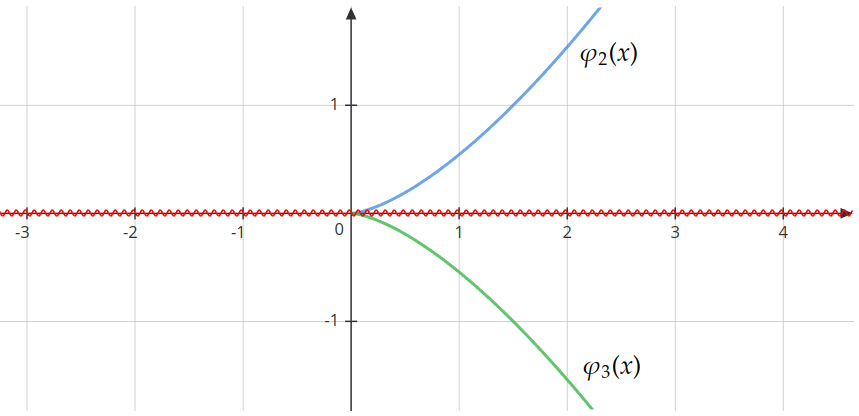
\includegraphics[width=\textwidth*2/3]{cauchy-esempio-unicita-soluzioni}
    \end{center}

    \(\implies{}\) dunque la soluzione non è unica.

\end{proof}

\pagebreak{}

\subsubsection{Lineare indipendenza}

Siano \(y_1(x)\) e \(y_2(x)\) due soluzioni di una EDO di I ordine lineare.

\(y_1(x)\) e \(y_2(x)\) si dicono linearmente indipendenti in I se presa una loro combinazione lineare e ponendola uguale a 0, l'unica soluzione è \(c_1=c_2=0\).

Ovvero:

\[
    c_1y_1(x) +c_2y_2(x) = 0 \iff c_1=c_2=0
\]

\subsubsection{Esercizi}

\subsubsection*{Esercizio 1}

\[
    y(x) = ce ^{x^{2}-x}+e ^{x^{2}-x}\int xe^{x} \diff x = c e ^{x^{2}-x}+xe ^{x^{2}}-e ^{x^{2}}
\]

Ponendo le condizioni di Cauchy:

\[
    y(0)=2
\]

La soluzione è:

\[
    2 e ^{x^{2}-x}+xe ^{x^{2}}-e ^{x^{2}}
\]

\subsubsection*{Esercizio 2}

\[
    y'=\sqrt[3]{x}y^{2}
\]

Una soluzione è:

\[
    y=0
\]

Le altre le trovo facendo l'integrale di:

\[
    \int \frac{1}{y^{2}} \diff y = \int \sqrt[3]{x} \diff x
\]

quindi \(y(x)\):

\[
    y(x)  = \frac{4}{3 \sqrt[3]{x^{4}}+c}
\]

impongo le condizioni e trovo c:

\[
    y(0) = \frac{-4}{0+c} = 2
\]

\[
    c = -2
\]

dunque la soluzione è:

\[
    y(x) = -\frac{4}{3 \sqrt[3]{x^{4}} - 2}
\]

il denominatore deve essere \(\neq 0\):

\[
    3 \sqrt[3]{x^{4}} - 2 \neq 0
\]

quindi:

\[
    x \neq (\frac{2}{3}^{ \frac{3}{4}})
\]

Il più ampio intervallo è:

\[
    0 \in \left(-\infty, \frac{2}{3}^{ \frac{3}{4}}\right)
\]
